%!TEX program = xelatex
\documentclass[11pt]{beamer}

\usepackage{amsfonts}
\usepackage{amsmath}
\usepackage{blindtext}
\usepackage{enumitem}
\usepackage{fancyvrb}
\usepackage{tikz}

\usetheme{SaoPaulo}

\title{Python Applications}
\subtitle{debugging code, solving problems}
\author{CS101 Lecture \#14}
\date{2016-11-16}

\setcounter{showSlideNumbers}{1}

\newcommand{\correctstar}{\textcolor{red}{$\star$}}

\begin{document}
  \setcounter{showProgressBar}{0}
  \setcounter{showSlideNumbers}{0}

%%%%%%%%%%%%%%%%%%%%%%%%%%%%%%%%%%%%%%%%%%%%%%%%%%%%%%%%%%%%%%%%%%%%%%%%%%%%%%%%
\frame{\titlepage}

%%%%%%%%%%%%%%%%%%%%%%%%%%%%%%%%%%%%%%%%%%%%%%%%%%%%%%%%%%%%%%%%%%%%%%%%%%%%%%%%
\setcounter{framenumber}{0}
\setcounter{showProgressBar}{1}
\setcounter{showSlideNumbers}{1}

%%%%%%%%%%%%%%%%%%%%%%%%%%%%%%%%%%%%%%%%%%%%%%%%%%%%%%%%%%%%%%%%%%%%%%%%%%%%%%%%
\section{Administrivia}

%%%%%%%%%%%%%%%%%%%%%%%%%%%%%%%%%%%%%%%%%%%%%%%%%%%%%%%%%%%%%%%%%%%%%%%%%%%%%%%%
\begin{frame}
  \frametitle{Administrivia}
  \Enlarge

  \begin{itemize}
  \myitem  Homework \#6 is due Today, Nov.\ 16.
  \myitem Prof. Li Er-Ping and Prof. Philip Krein will be out of town tomorrow, so I will (very happily) show up -- \emph{again} -- on tomorrow's ENG100 course.
  \myitem  Any questions for the lab sessions? suggestions or critiques?
  %\myitem  Office hours will change from Wed to Thu next week (check website).
  \end{itemize}
\end{frame}

%%%%%%%%%%%%%%%%%%%%%%%%%%%%%%%%%%%%%%%%%%%%%%%%%%%%%%%%%%%%%%%%%%%%%%%%%%%%%%%%
\iffalse

\begin{frame}[fragile]
  \frametitle{Brief Note on Directories}
  \Enlarge

  \begin{itemize}
  \myitem  Directories are written before the file name:
    \begin{Verbatim}
'/Users/davis68/cs101/hw07/batting.csv'
'C:/cs101/hw07/batting.csv'  # note / not \
    \end{Verbatim}
  \myitem  These are \emph{absolute} paths (where the file is on the machine)---these always begin with \texttt{/} (Linux/Mac) or \texttt{X:} (Windows).
  \end{itemize}
\end{frame}

%%%%%%%%%%%%%%%%%%%%%%%%%%%%%%%%%%%%%%%%%%%%%%%%%%%%%%%%%%%%%%%%%%%%%%%%%%%%%%%%
\begin{frame}[fragile]
  \frametitle{Brief Note on Directories}
  \Enlarge

  \begin{itemize}
  \myitem  Relative paths are often more convenient:
    \begin{Verbatim}
'batting.csv'
'./batting.csv'  # . is current directory
'../hw07/batting.csv'  # .. is parent dir
    \end{Verbatim}
  \myitem  For 101, we recommend putting the file in the same directory (use the code from last time).
  \end{itemize}
\end{frame}

\fi

%%%%%%%%%%%%%%%%%%%%%%%%%%%%%%%%%%%%%%%%%%%%%%%%%%%%%%%%%%%%%%%%%%%%%%%%%%%%%%%%
\section{Warmup Quiz}

%%%%%%%%%%%%%%%%%%%%%%%%%%%%%%%%%%%%%%%%%%%%%%%%%%%%%%%%%%%%%%%%%%%%%%%%%%%%%%%%
\begin{frame}[fragile]
  \frametitle{Question \#1}
  \Enlarge

  \begin{Verbatim}
a = [ 'alpha','beta','gamma' ]
b = [ 2,3,4 ]
for i,j in enumerate( a ):
    print( i,j )
  \end{Verbatim}

  Which of the following answers is a possible line of output of the above code?

  \begin{enumerate}[label=\Alph*]
  \item  \texttt{4 gamma}
  \item  \texttt{2 gamma}
  \item  \texttt{gamma 4}
  \item  \texttt{gamma 2}
  \end{enumerate}
  
  (\emph{What does the English word ``enumerate'' mean, and the function definition in python?})
\end{frame}

%%%%%%%%%%%%%%%%%%%%%%%%%%%%%%%%%%%%%%%%%%%%%%%%%%%%%%%%%%%%%%%%%%%%%%%%%%%%%%%%
\begin{frame}[fragile]
  \frametitle{Question \#1}
  \Enlarge

  \begin{Verbatim}
a = [ 'alpha','beta','gamma' ]
b = [ 2,3,4 ]
for i,j in enumerate( a ):
    print( i,j )
  \end{Verbatim}

  Which of the following answers is a possible line of output of the above code?

  \begin{enumerate}[label=\Alph*]
  \item  \texttt{4 gamma}
  \item  \texttt{2 gamma}  \correctstar
  \item  \texttt{gamma 4}
  \item  \texttt{gamma 2}
  \end{enumerate}
  
\end{frame}

%%%%%%%%%%%%%%%%%%%%%%%%%%%%%%%%%%%%%%%%%%%%%%%%%%%%%%%%%%%%%%%%%%%%%%%%%%%%%%%%
\begin{frame}[fragile]
  \frametitle{Question \#2}
  \Enlarge

  \begin{Verbatim}
a = [ 'alpha','beta','gamma' ]
b = [ 2,3,4 ]
for i,j in zip( a,b ):
    print( i,j )
  \end{Verbatim}

  Which of the following answers is a possible line of output of the above code?

  \begin{enumerate}[label=\Alph*]
  \item  \texttt{4 gamma}
  \item  \texttt{2 gamma}
  \item  \texttt{gamma 4}
  \item  \texttt{gamma 2}
  \end{enumerate}
\end{frame}

%%%%%%%%%%%%%%%%%%%%%%%%%%%%%%%%%%%%%%%%%%%%%%%%%%%%%%%%%%%%%%%%%%%%%%%%%%%%%%%%
\begin{frame}[fragile]
  \frametitle{Question \#2}
  \Enlarge

  \begin{Verbatim}
a = [ 'alpha','beta','gamma' ]
b = [ 2,3,4 ]
for i,j in zip( a,b ):
    print( i,j )
  \end{Verbatim}

  Which of the following answers is a possible line of output of the above code?

  \begin{enumerate}[label=\Alph*]
  \item  \texttt{4 gamma}
  \item  \texttt{2 gamma}
  \item  \texttt{gamma 4}  \correctstar
  \item  \texttt{gamma 2}
  \end{enumerate}
  
   (\emph{What if b =  [2,3,4,5]?})
\end{frame}

%%%%%%%%%%%%%%%%%%%%%%%%%%%%%%%%%%%%%%%%%%%%%%%%%%%%%%%%%%%%%%%%%%%%%%%%%%%%%%%%
\section{When Things Go Wrong}

%%%%%%%%%%%%%%%%%%%%%%%%%%%%%%%%%%%%%%%%%%%%%%%%%%%%%%%%%%%%%%%%%%%%%%%%%%%%%%%%
% full-slide image
{ \setbeamertemplate{navigation symbols}{}
    \begin{frame}[plain]
        \begin{tikzpicture}[remember picture,overlay]
            \node[at=(current page.center)] {
                
\includegraphics[height=\paperheight]{./img/despair.jpg}
            };
        \end{tikzpicture}
        My code doesn’t work.
     \end{frame}
}

%%%%%%%%%%%%%%%%%%%%%%%%%%%%%%%%%%%%%%%%%%%%%%%%%%%%%%%%%%%%%%%%%%%%%%%%%%%%%%%%
% full-slide image
{ \setbeamertemplate{navigation symbols}{}
    \begin{frame}[plain]
        \begin{tikzpicture}[remember picture]
            \node[at=(current page.center)] {
                
\includegraphics[height=0.8\paperheight]{./img/einstein.jpg}
            };
        \end{tikzpicture}
        
        \Enlarge
        errors are cute
     \end{frame}
}

{ \setbeamertemplate{navigation symbols}{}
    \begin{frame}[plain]
    	My experience with errors:
	\begin{enumerate}
         \myitem  You never learn to program correctly without making errors
        
         \myitem  Some errors reveal the discrepancies between your way of thinking and the machine's logic
        
         \myitem  A genuine intuition is always error-free -- you make errors when you start to \emph{think}.
        \end{enumerate}
     
     \end{frame}
}

%%%%%%%%%%%%%%%%%%%%%%%%%%%%%%%%%%%%%%%%%%%%%%%%%%%%%%%%%%%%%%%%%%%%%%%%%%%%%%%%
\begin{frame}[fragile]
  \frametitle{Debugging}
  \Enlarge
  
  How do I know it isn’t working?
  \begin{enumerate}
  \myitem  What do I expect it to do?
  \myitem  What is my code doing instead?
  \myitem  How to identify the source of error and Fix it? 
  \end{enumerate}
  \hspace{8mm}==> Debugging
\end{frame}



%%%%%%%%%%%%%%%%%%%%%%%%%%%%%%%%%%%%%%%%%%%%%%%%%%%%%%%%%%%%%%%%%%%%%%%%%%%%%%%%
\begin{frame}[fragile]
  \frametitle{Debugging}
  \Enlarge

  \begin{enumerate}
  \myitem  A few working definitions:
  \begin{enumerate}
    \mysubitem  \textbf{Exceptions}--- unusual behaviors occurred in the execution of a program; caught by a try:\{...\}except e:\{...\} syntax. Most languages (Python, C++, Java) have this. \pause
    \mysubitem  \textbf{Errors}--- exceptions that cause the program to be unrunnable  \pause
    \mysubitem  \textbf{Traceback}---listing of function calls on the stack at the time the exception (error) arises \pause
    \mysubitem  \textbf{Bugs}---errors and exceptions, but also miswritten, ambiguous, or incorrect code which in fact runs but does not advertise its miscreancy
    \end{enumerate}
  \end{enumerate}
\end{frame}

%%%%%%%%%%%%%%%%%%%%%%%%%%%%%%%%%%%%%%%%%%%%%%%%%%%%%%%%%%%%%%%%%%%%%%%%%%%%%%%%
\begin{frame}[fragile]
  \frametitle{Common exceptions}
  \Enlarge

  \begin{enumerate}
  \myitem  \texttt{SyntaxError}
  \myitem  \texttt{NameError}
  \myitem  \texttt{TypeError}
  \myitem  \texttt{ValueError}
  \myitem  \texttt{IOError}
  \myitem  \texttt{IndexError}
  \myitem  \texttt{KeyError}
  \myitem  \texttt{ZeroDivisionError}
  \myitem  \texttt{IndentationError}
  \myitem  \texttt{Exception: subsumes all above and many others}
  \end{enumerate}
\end{frame}

%%%%%%%%%%%%%%%%%%%%%%%%%%%%%%%%%%%%%%%%%%%%%%%%%%%%%%%%%%%%%%%%%%%%%%%%%%%%%%%%
\begin{frame}[fragile]
  \frametitle{Common exceptions}
  \Enlarge

  \begin{enumerate}
  \myitem \texttt{SyntaxError}---check missing colons or parentheses
  \myitem \texttt{NameError}---check for typos, function definitions
  \myitem \texttt{TypeError}---check variable types (coerce if necessary)
  \myitem \texttt{ValueError}---check function parameters
  \myitem \texttt{IOError}---check that files exist
  \end{enumerate}
\end{frame}

%%%%%%%%%%%%%%%%%%%%%%%%%%%%%%%%%%%%%%%%%%%%%%%%%%%%%%%%%%%%%%%%%%%%%%%%%%%%%%%%
\begin{frame}[fragile]
  \frametitle{Common exceptions}
  \Enlarge

  \begin{enumerate}
  \myitem \texttt{IndexError}---don't reference nonexistent list elements
  \myitem \texttt{KeyError}---similar to an IndexError, but for dictionaries
  \myitem  \texttt{ZeroDivisionError}---three guesses...
  \myitem  \texttt{IndentationError}---check that spaces and tabs aren't mixed
  \myitem  \texttt{Exception}---generic error category
  \end{enumerate}
\end{frame}

%%%%%%%%%%%%%%%%%%%%%%%%%%%%%%%%%%%%%%%%%%%%%%%%%%%%%%%%%%%%%%%%%%%%%%%%%%%%%%%%
\begin{frame}[fragile]
  \frametitle{Comprehension Question}
  \Enlarge

  \begin{Verbatim}
# calculate squares
d = list(range(10))
while i < 10:
    d[i] = d[i] ** 2.0
    i += 1
  \end{Verbatim}

  Which error would this code produce?

  \begin{enumerate}[label=\Alph*]
  \item  SyntaxError
  \item  IndexError
  \item  ValueError
  \item  NameError
  \end{enumerate}
\end{frame}

%%%%%%%%%%%%%%%%%%%%%%%%%%%%%%%%%%%%%%%%%%%%%%%%%%%%%%%%%%%%%%%%%%%%%%%%%%%%%%%%
\begin{frame}[fragile]
  \frametitle{Comprehension Question}
  \Enlarge

  Which of the following would produce \texttt{TypeError}?

  \begin{enumerate}[label=\Alph*]
  \item  \begin{verbatim}'2' + 2\end{verbatim}
  \item  \begin{verbatim}2 / 0\end{verbatim}
  \item  \begin{verbatim}2e8 + (1+0j)\end{verbatim}
  \item  \begin{verbatim}'2' * 2\end{verbatim}
  \end{enumerate}
\end{frame}

%%%%%%%%%%%%%%%%%%%%%%%%%%%%%%%%%%%%%%%%%%%%%%%%%%%%%%%%%%%%%%%%%%%%%%%%%%%%%%%%
\begin{frame}[fragile]
  \frametitle{Program stack}

  \begin{tabular}{cc}
    \begin{minipage}{2in}
    \begin{verbatim}
# in file `main.py`
def do_numerics():
    print(sin(5.0))

do_numerics()
    \end{verbatim}
    \end{minipage}
    &
    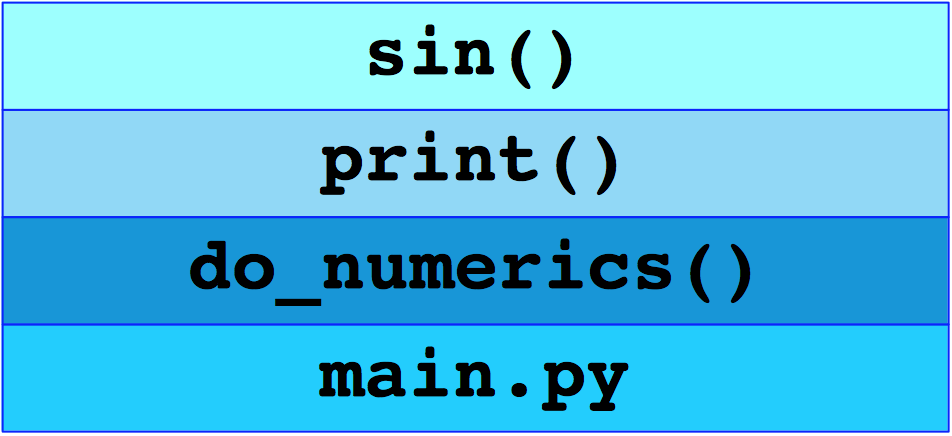
\includegraphics[width=0.5\textwidth]{./img/stack.png}
    \\
  \end{tabular}
\end{frame}

%(you do the same thing when you start cleaning your room, and then you have to set that context aside and clean your bed, and set that context aside and wash your sheets, and set that context aside and run out for detergent)

%%%%%%%%%%%%%%%%%%%%%%%%%%%%%%%%%%%%%%%%%%%%%%%%%%%%%%%%%%%%%%%%%%%%%%%%%%%%%%%%
\begin{frame}[fragile]
  \frametitle{Program stack trace}

  \begin{Verbatim}
Traceback (most recent call last):
    File "main.py", line 7, in <module>
      do_numerics()
    File "main.py", line 4, in do_numerics
      print(sin(5.0))
NameError: name 'sin' is not defined
  \end{Verbatim}

  \begin{tabular}{cc}
  \begin{minipage}{2in}
  \begin{enumerate}
  \myitem  Read these from end to beginning:
  \mysubitem  \texttt{sin} in \texttt{do\_numerics} in file \texttt{main.py}
  \end{enumerate}
  \end{minipage}
  &
  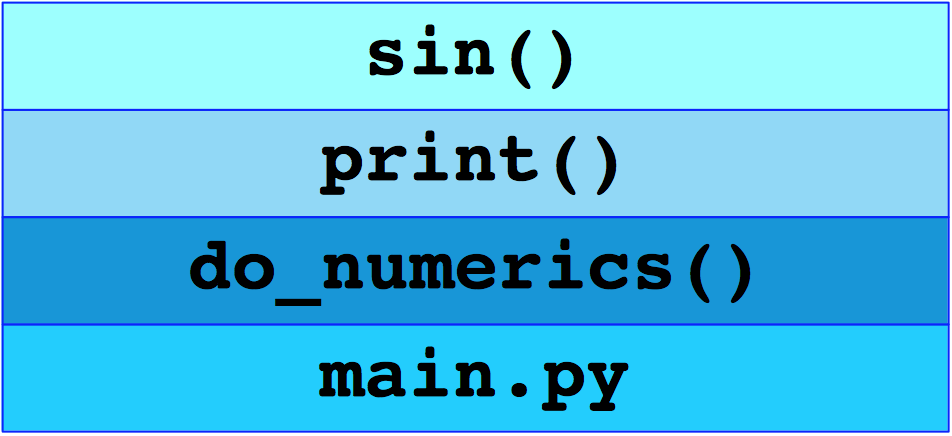
\includegraphics[width=0.5\textwidth]{./img/stack.png}\\
  \end{tabular}
\end{frame}

%%%%%%%%%%%%%%%%%%%%%%%%%%%%%%%%%%%%%%%%%%%%%%%%%%%%%%%%%%%%%%%%%%%%%%%%%%%%%%%%
\section{Debugging}

%%%%%%%%%%%%%%%%%%%%%%%%%%%%%%%%%%%%%%%%%%%%%%%%%%%%%%%%%%%%%%%%%%%%%%%%%%%%%%%%
\begin{frame}[fragile]
  \frametitle{Debugging}
  \Enlarge

Brian Kernighan:

``Debugging is twice as hard as writing the code in the first place. Therefore, if you write the code as cleverly as possible, you are, by definition, not smart enough to debug it.''
\end{frame}

%%%%%%%%%%%%%%%%%%%%%%%%%%%%%%%%%%%%%%%%%%%%%%%%%%%%%%%%%%%%%%%%%%%%%%%%%%%%%%%%
\begin{frame}[fragile]
  \frametitle{Debugging example}

  This code should find all lines in a file whose first two letters are the same:
  \begin{Verbatim}[commandchars=\\\{\},commentchar=\%]
for line in open( "words.txt" ):
    line = line.strip()
    if len( line ) >= 2:
        a,b = line[1:3]
    if a == b:
        print( line )
  \end{Verbatim}
\end{frame}

%%%%%%%%%%%%%%%%%%%%%%%%%%%%%%%%%%%%%%%%%%%%%%%%%%%%%%%%%%%%%%%%%%%%%%%%%%%%%%%%
\begin{frame}[fragile]
  \frametitle{Debugging example}

  This code should find all lines in a file whose first two letters are the same:
  \begin{Verbatim}[commandchars=\\\{\},commentchar=\%]
for line in open( "words.txt" ):
    line = line.strip()
    if len( line ) >= 2:
        \textcolor{CS101GradTop}{print( line )}
        a,b = line[1:3]
        \textcolor{CS101GradTop}{print( a,b )}
    if a == b:
        print( line )
  \end{Verbatim}
\end{frame}

%%%%%%%%%%%%%%%%%%%%%%%%%%%%%%%%%%%%%%%%%%%%%%%%%%%%%%%%%%%%%%%%%%%%%%%%%%%%%%%%
\begin{frame}[fragile]
  \frametitle{Debugging example}

  This code should find all lines in a file whose first two letters are the same:
  \begin{Verbatim}[commandchars=\\\{\},commentchar=\%]
for line in open( "words.txt" ):
    line = line.strip()
    if len( line ) >= 2:
        a,b = line[\textcolor{CS101GradTop}{0:2}]
    if a == b:
        print( line )
  \end{Verbatim}
\end{frame}

\begin{frame}[fragile]
  \frametitle{Debugging example}

  This code should find all lines in a file whose first two letters are the same:
  \begin{Verbatim}[commandchars=\\\{\},commentchar=\%]
for line in open( "words.txt" ):
    line = line.strip()
    if len( line ) >= 2:
        a,b = line[0:2]
    \textcolor{CS101GradTop}{if a == b:}
        print( line )
  \end{Verbatim}
\end{frame}

%(this doesn't tell you where to go, but does tell you if how you're going is valid)

%%%%%%%%%%%%%%%%%%%%%%%%%%%%%%%%%%%%%%%%%%%%%%%%%%%%%%%%%%%%%%%%%%%%%%%%%%%%%%%%
\iffalse
\begin{frame}[fragile]
  \frametitle{Debugging strategies}
  \Enlarge

  \begin{enumerate}
  \myitem  When do things go wrong? %\pause
  \myitem  Three categories of problems:
    \begin{enumerate}
    \mysubitem  before the code runs
    \mysubitem  while the code is running
    \mysubitem  in the results
    \end{enumerate}
  \end{enumerate}
\end{frame}
\fi
%%%%%%%%%%%%%%%%%%%%%%%%%%%%%%%%%%%%%%%%%%%%%%%%%%%%%%%%%%%%%%%%%%%%%%%%%%%%%%%%
\begin{frame}[fragile]
  \frametitle{Debugging strategies}
  \Enlarge

  \begin{enumerate}
  \myitem  Start early. %\pause
  \myitem  Read the problem statement carefully. %\pause
  \myitem  Add print statements. %\pause
  \myitem  Chart the flow of the program. %\pause
  \myitem  Break the program down into functions. %\pause
  \myitem  Document functions before writing them. %\pause
  \myitem  Show it to someone else. People have blindspots. %\pause
  \myitem  Make no assumptions! If your thinking is not precise, your code will not be precise. %\pause
  \myitem  Start over from scratch. Take a fresh look at the problem.
  \end{enumerate}
\end{frame}

\begin{frame}[fragile]
  \frametitle{Debugging strategies}
  \Enlarge

  \begin{enumerate}
  \myitem  Start early. %\pause
  \myitem  Read the problem statement carefully. %\pause
  \myitem  \textcolor{CS101GradTop}{Add print statements.} %\pause
  \myitem  Chart the flow of the program. %\pause
  \myitem  Break the program down into functions. %\pause
  \myitem  Document functions before writing them. %\pause
  \myitem  \textcolor{CS101GradTop}{Show it to someone else. Everyone has a blind spots someone else can easily see.} %\pause
  \myitem  Make no assumptions! If your thinking is not precise, your code will not be precise. %\pause
  \myitem  Start over from scratch. Take a fresh look at the problem.
  \end{enumerate}
\end{frame}

%%%%%%%%%%%%%%%%%%%%%%%%%%%%%%%%%%%%%%%%%%%%%%%%%%%%%%%%%%%%%%%%%%%%%%%%%%%%%%%%
%\begin{frame}[fragile]
%  \frametitle{Debugging strategies}
%  \Enlarge

%  Consider the following series statement for a Bessel function of the first kind,
%  $$J_{0}(x) = \sum_{m=0}^{\infty} \frac{(-1)^{m}}{m! (m+1)!} {\left(\frac{x}{2}\right)}^{2m} \text{.} $$
%\end{frame}

%debug bessel function
%debug Neetesh's code

%%%%%%%%%%%%%%%%%%%%%%%%%%%%%%%%%%%%%%%%%%%%%%%%%%%%%%%%%%%%%%%%%%%%%%%%%%%%%%%%
\section{Style}

%%%%%%%%%%%%%%%%%%%%%%%%%%%%%%%%%%%%%%%%%%%%%%%%%%%%%%%%%%%%%%%%%%%%%%%%%%%%%%%%
\begin{frame}[fragile]
  \frametitle{Style}
  \Enlarge

  \begin{enumerate}
  \myitem  What makes a good Python code? %\pause
  \end{enumerate}
  \begin{center}
    \textcolor{CS101Base}{\Huge \texttt{import this}}
  \end{center}
\end{frame}

%%%%%%%%%%%%%%%%%%%%%%%%%%%%%%%%%%%%%%%%%%%%%%%%%%%%%%%%%%%%%%%%%%%%%%%%%%%%%%%%

\begin{frame}[fragile]
  \frametitle{Style}
  \Enlarge

  \begin{enumerate}
  \myitem  Use descriptive variable names. %\pause
  \myitem  Why do we write comments? %\pause
  \myitem  For the person who next looks at the code!
  \begin{Verbatim}
x_vals = [0,0.1,0.2,0.3,0.4]  # meters
faraday = 96485.3328959  # coulombs,
                         # electric charge
  \end{Verbatim}
  \end{enumerate}
\end{frame}

%%%%%%%%%%%%%%%%%%%%%%%%%%%%%%%%%%%%%%%%%%%%%%%%%%%%%%%%%%%%%%%%%%%%%%%%%%%%%%%%

\begin{frame}[fragile]
  \frametitle{Style}
  \Enlarge

  \begin{enumerate}
  \myitem  Document your code!
  \myitem  Every function should have a docstring.
  \end{enumerate}
  \begin{Verbatim}
def warning( msg ):
    '''Display a warning message.'''
    print( 'Warning:  %s'%msg)
  \end{Verbatim}
  %\pause
  \begin{enumerate}
  \myitem  Docstrings explain what the function does and what its parameters are.
  \myitem  They always are triple-quoted strings on the first line of the function block.
  \end{enumerate}
  %\pause
  \begin{Verbatim}
help(warning)
  \end{Verbatim}
\end{frame}

%%%%%%%%%%%%%%%%%%%%%%%%%%%%%%%%%%%%%%%%%%%%%%%%%%%%%%%%%%%%%%%%%%%%%%%%%%%%%%%%
\begin{frame}[fragile]
  \frametitle{Style}
  \Enlarge

  \begin{enumerate}
  \myitem  Use functions to structure code (also called code refactoring).
  \myitem  This makes code more readable (and debuggable!).
  \myitem  A \texttt{main} function lets you organize your program's logic succinctly.
  \end{enumerate}
\end{frame}


%%%%%%%%%%%%%%%%%%%%%%%%%%%%%%%%%%%%%%%%%%%%%%%%%%%%%%%%%%%%%%%%%%%%%%%%%%%%%%%%
\begin{frame}[fragile]
  \frametitle{Style}
  \Enlarge

  \begin{enumerate}
  \myitem  A \texttt{main} function lets you organize your program's logic succinctly.
  \myitem  We have a special way of writing these so that we can load our code as a module or execute it alone.
  \myitem  A module's '\_\_name\_\_' (a built-in variable) is set to '\_\_main\_\_' when it is executed as a script, but not when it is {\emph imported}
  \end{enumerate}
  \begin{Verbatim}
def main():
    # your code here

if __name__ == '__main__':
    main()
  \end{Verbatim}
\end{frame}

%heat_eqn_cl.py (in functions, not)
%Compare commented/uncommented code

%%%%%%%%%%%%%%%%%%%%%%%%%%%%%%%%%%%%%%%%%%%%%%%%%%%%%%%%%%%%%%%%%%%%%%%%%%%%%%%%
\begin{frame}
  \frametitle{Course outline}
  \Enlarge

  Course Summary:
  \begin{itemize}
  \item  Python basics:
    \begin{itemize}
    \item  operators, expressions, data types, data structures
    \end{itemize}
  \item  Python applications:
    \begin{itemize}
    \item  workflow, I/O, \correctstar debugging
    \end{itemize}
  \item  Scientific Python:
    \begin{itemize}
    \item  plotting, calculating, modeling, simulation, optimization
    \end{itemize}
  \item  MATLAB:
    \begin{itemize}
    \item  recap of the above
    \end{itemize}
  \end{itemize}

  \correctstar (you are here)
\end{frame}

%%%%%%%%%%%%%%%%%%%%%%%%%%%%%%%%%%%%%%%%%%%%%%%%%%%%%%%%%%%%%%%%%%%%%%%%%%%%%%%%
\iffalse
\section{Reminders}

%%%%%%%%%%%%%%%%%%%%%%%%%%%%%%%%%%%%%%%%%%%%%%%%%%%%%%%%%%%%%%%%%%%%%%%%%%%%%%%%
\begin{frame}
  \frametitle{Reminders}
  \Enlarge

  \begin{itemize}
  \myitem  Homework \#7 is due Monday, Oct.\ 17.
  \myitem  Midterm reflection exercise on website for extra credit (through Friday).
  \myitem  Office hours will change from Wed to Thu next week (check website).
  \end{itemize}
\end{frame}

\fi

\end{document}
